\newpage
%========================================================[DETERMINISTIC ANALYSIS]
\section{DETERMINISTIC ANALYSIS}


%=========================================================[BEACH ANALYSIS
\subsection{COASTAL ANALYSIS}

The non-linear forecasting technique is applied independently to the pre-nourishment and post-nourishment intertidal beach profiles (Figure \ref{beach}). The $R^2$ values are shown in Figure \ref{beach_contour_raw}.

\begin{figure}[htbp] %  figure placement: here, top, bottom, or page
   \centering
   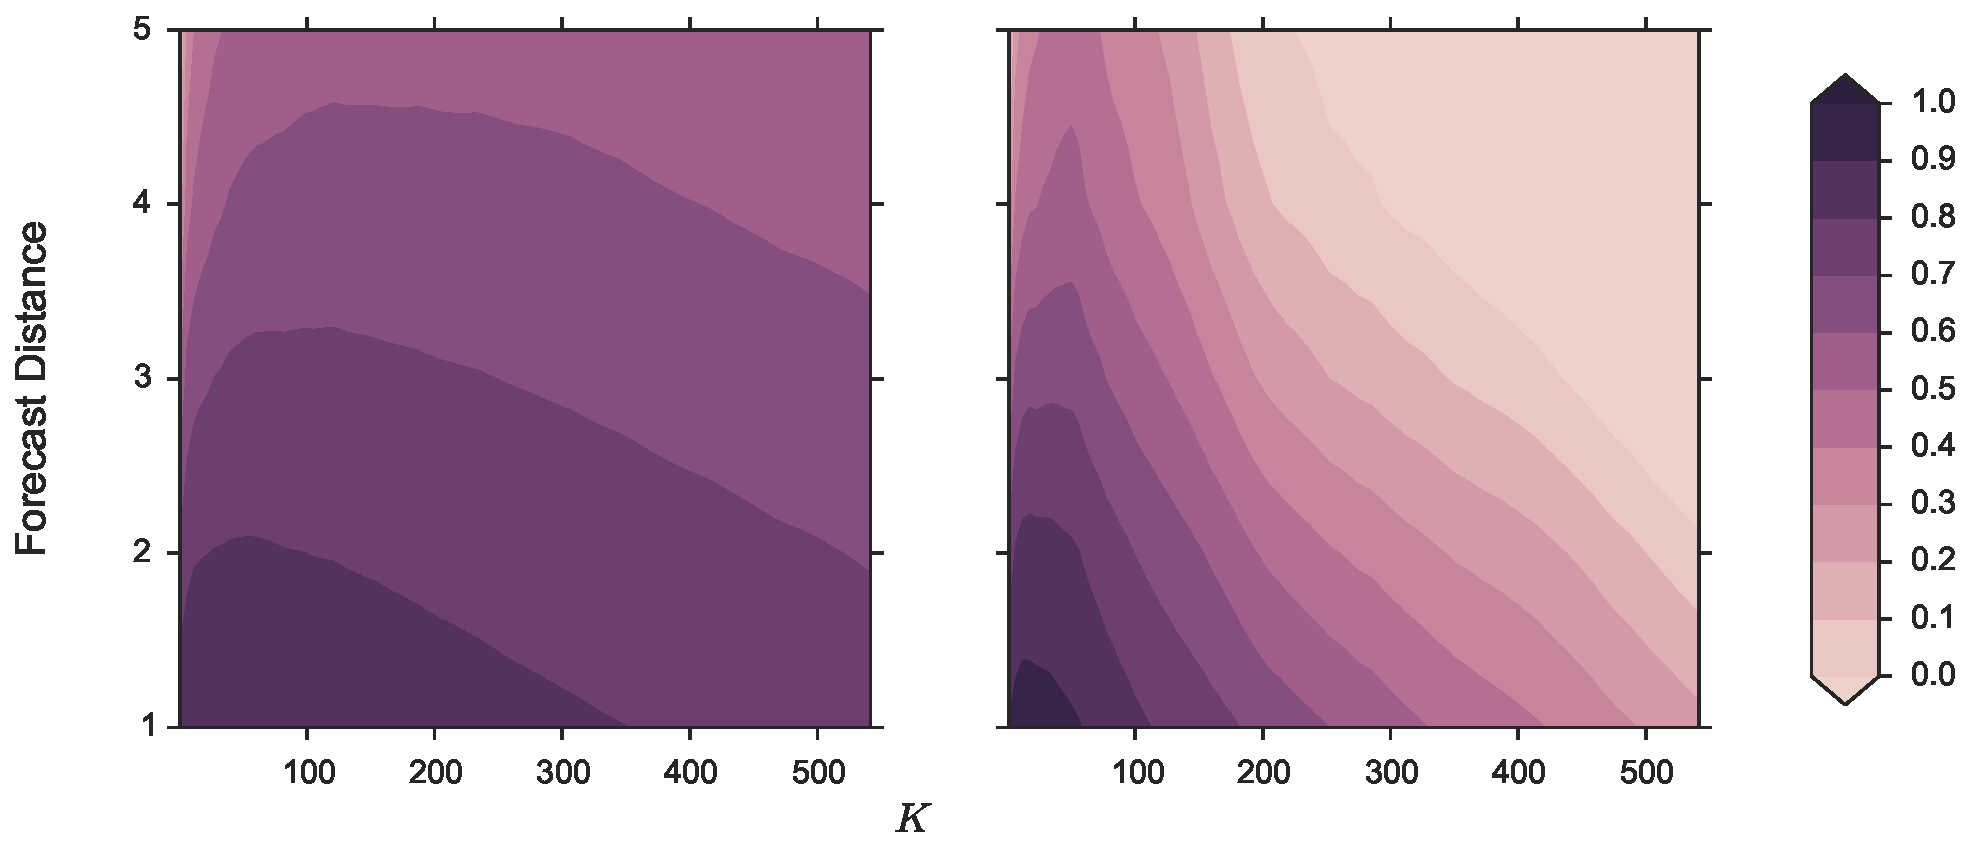
\includegraphics[height=2in]{beach/beach_contour_raw.pdf} 
   \caption{Non-linear forecasting results for the pre-nourishment beach (left) and post-nourishment beach (right). The coefficient of determination, $R^2$, is plotted against near neighbors ($K$) and forecast distance.}
   \label{beach_contour_raw}
\end{figure}


The non-linear forecasting results show two very different trends. For the pre-nourishment beach, the $R^2$ values drop off more slowly than the post-nourishment beach for both forecast distance and near neighbors. One interpretation of the results for the pre-nourishment beach is that the high forecast skill over a relatively wide range of low $K$ and forecast distance indicates that the state space for the pre-nourishment beach is more populated than the post-nourishment beach.  Additionally, since forecast skill drops off more quickly for the post-nourishment beach, near neighbors in the state space do not evolve as similarly as the pre-nourishment beach. These trends seem to suggest that the nourishment episode abruptly moved the intertidal region away from its attractor and that it is slowly progressing back toward it's steady state and in doing so is dominated by internal system dynamics as opposed to responding to noisy forcing.

% Since the state space for the post-nourishment beach appears to be incomplete, the deterministic metric is not able to be calculated. Instead, to explore the day to day changes in the beach, the daily difference is calculated. The intent is to 



% \begin{figure}[htbp] %  figure placement: here, top, bottom, or page
%    \centering
%    \includegraphics[height=2.5in]{beach/beach_contour.pdf} 
%    \caption{Results of non-linear forecasting for the beach difference image. Color corresponds to the $R^2$ value.}
%    \label{beach_contour}
% \end{figure}

% \begin{figure}[htbp] %  figure placement: here, top, bottom, or page
%    \centering
%    \includegraphics[height=2.5in]{beach/beach_bar_plot.pdf} 
%    \caption{Deterministic metric calculated for the daily difference.}
%    \label{beach_bar}
% \end{figure}

%  Both images show a small peak at low number of near neighbors indicating that the system is deterministic and is not completely dominated by noise. The deterministic metric, however, indicates that the post-nourishment beach is slightly more deterministic than the pre-nourishment beach. This suggests that the large amount of fresh sand that was placed on the beach is more succeptible to internal dynamics. The sand is attempting to find a steady state and is more influenced by its shape than outside forcings such as waves.


%=========================================================[CORAL ANALYSIS]
\subsection{CORAL ANALYSIS}


The non-linear forecasting technique is applied to the coral images and the resulting contour plots of forecast skill are shown in Figure \ref{coral_contours}.

\begin{figure}[htbp] %  figure placement: here, top, bottom, or page
   \centering
   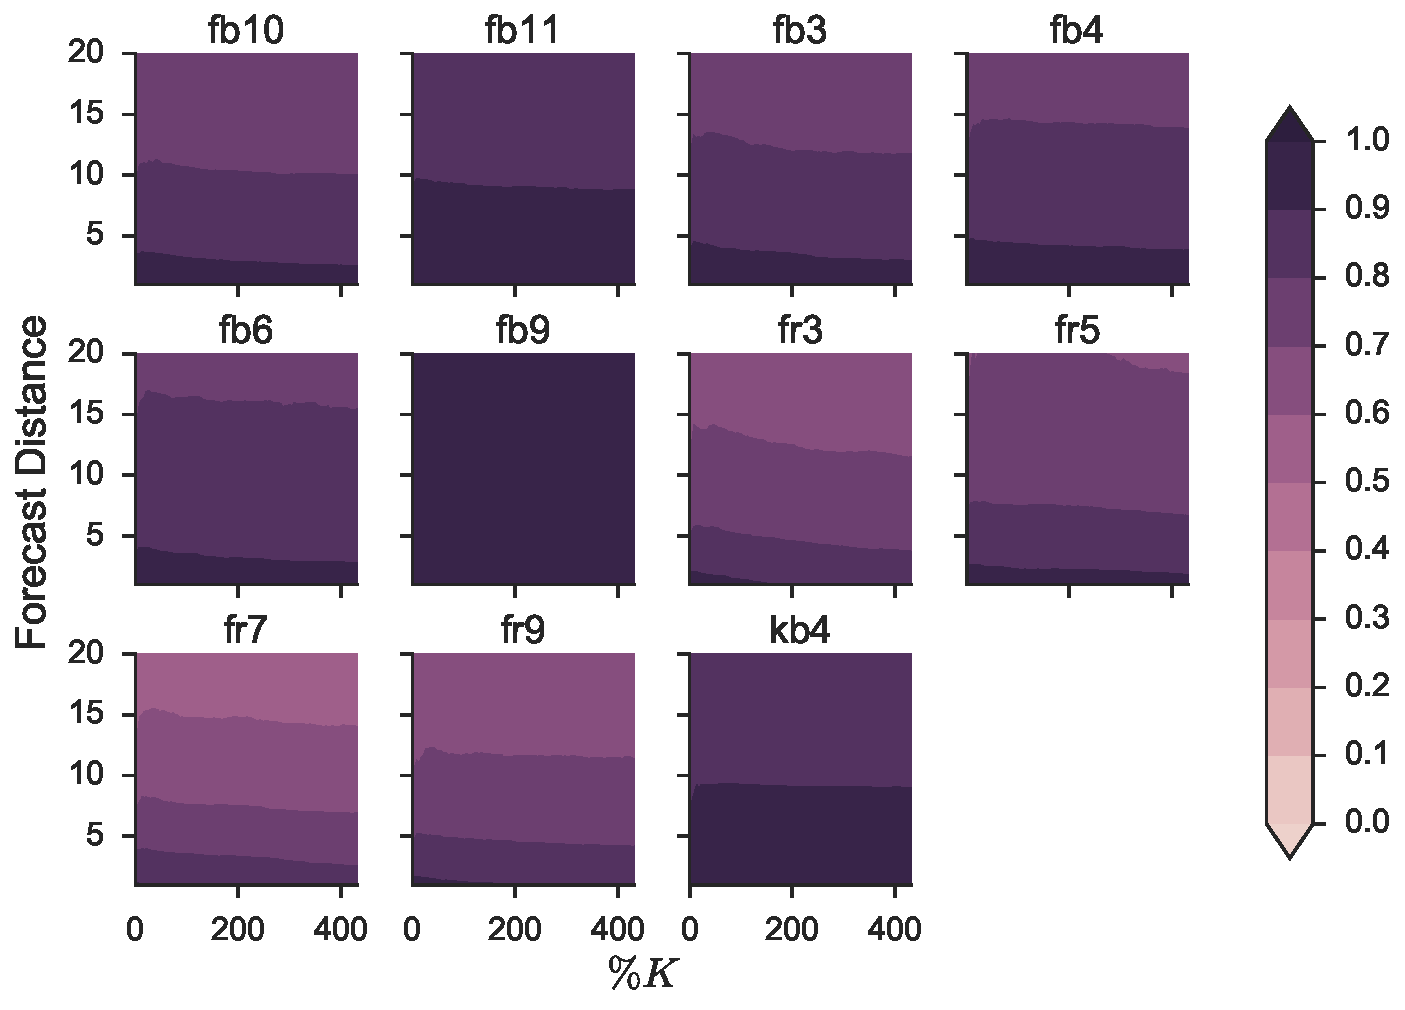
\includegraphics[width=5in]{coral/coral_contours.pdf} 
   \caption{Non-linear forecasting results for the coral zones. The percent correctly forecast, $P_c$, is plotted against near neighbors ($K$) and forecast distance.}
   \label{coral_contours}
\end{figure}

All zones display the same trend: highest $P_c$ values are obtained at low $K$ values and low forecast distances. This indicates that each zone is deterministic and that nearby regions in the reconstructed state space evolve similarly. Physically, this means that species on reefs influence the distribution of species around them. Assuming that all of zones are generated by the same dynamics (competition for benthic space between species on the coral reef) and that all of the state spaces are well populated, the deterministic metric can be compared across the various islands (Figure \ref{coral_bar}).
 
\begin{figure}[htbp] %  figure placement: here, top, bottom, or page
   \centering
   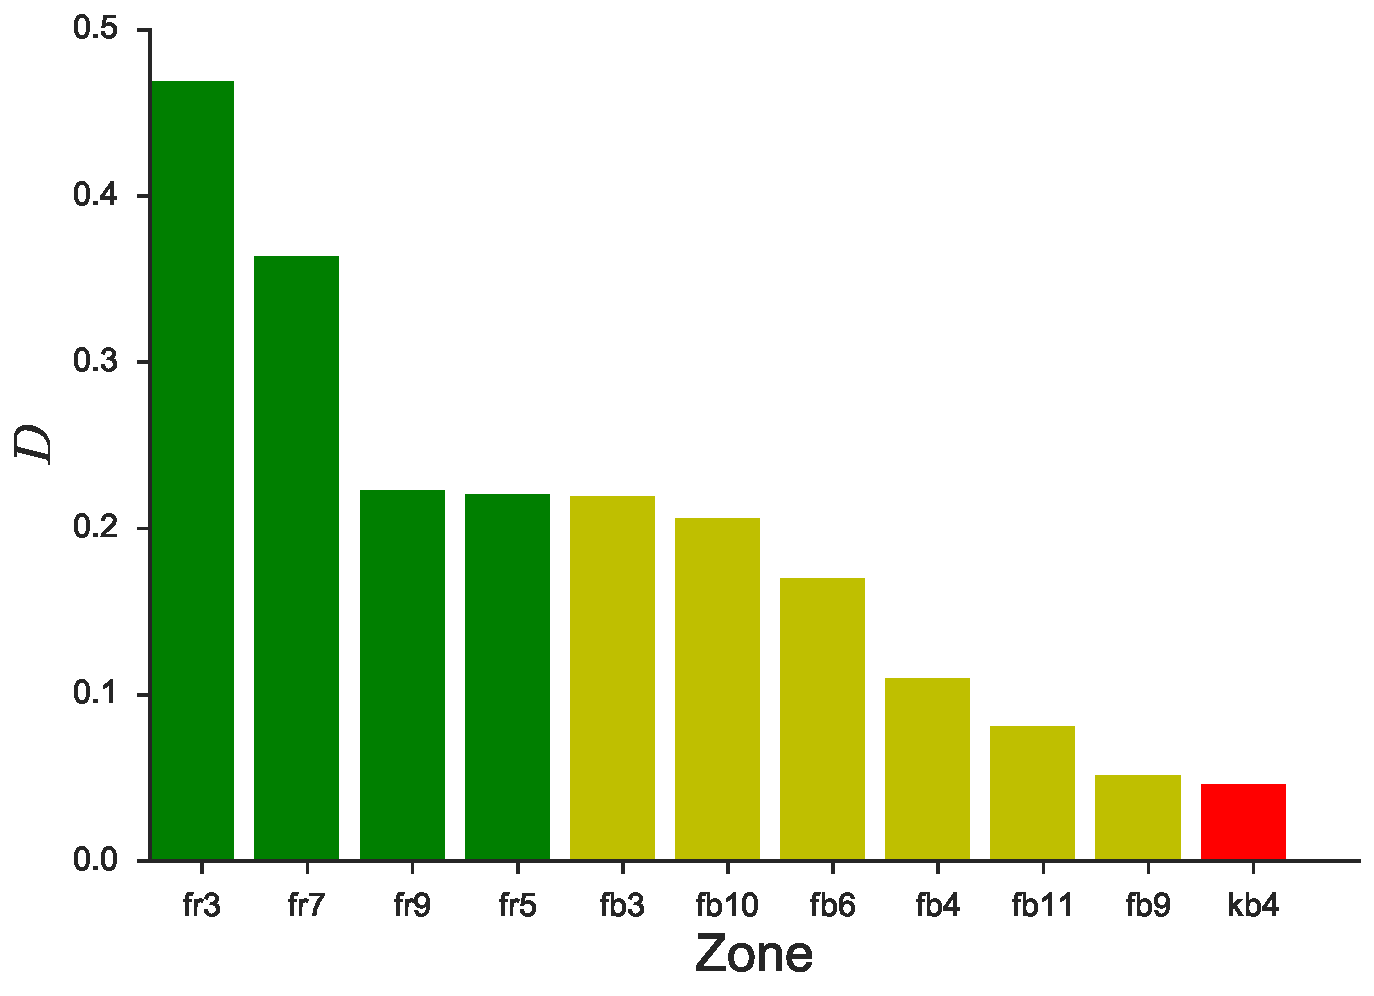
\includegraphics[width=5in]{coral/bar_plot_coral.pdf} 
   \caption{Deterministic metric, $D$, for the coral zones. The $x$-axis and color indicate location (green is Palmyra, yellow is Fanning, and red is Christmas).}
   \label{coral_bar}
\end{figure}

The metric shows a distinct trend with respect to each of the three islands with the highest values occurring at Palmyra. It appears as though the relatively pristine reefs of Palmyra have a more spatially deterministic structure, suggesting that non-linear internal spatial dynamics play a larger role in dictating benthic patterns at Palmyra than at the other islands in this study. The second grouping is four of the six Fanning Island zones. This indicates that there is still structure in the benthic patterning and that internal non-linear dynamics play a role in shaping the structure, but the relative influence of spatial noise is stronger than at Palmyra. The last grouping consists of three zones at Fanning and Christmas. These locations show  the least deterministic spatial structure according to the metric and these locations are in fact the most degraded of all the study zones. These results indicate that the non-linear forecasting technique coupled with the deterministic metric is able to distinguish relative reef health. This suggests that pollution and disturbance of the reef ecosystem destroys natural spatial relationships (non-linear internal dynamics) resulting in a benthic spatial structure that is more random.



